\section{Hexa--copter model}
\begin{marginfigure}
	\centering
	%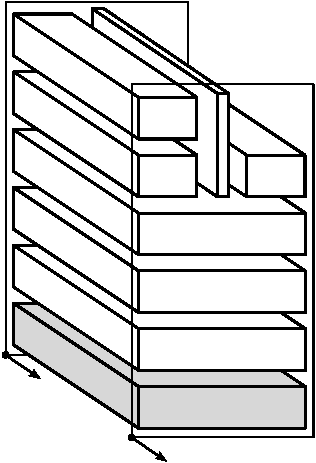
\includegraphics[scale=0.5]{ch3/img/PA_map_dynamic.pdf}
	\begin{tikzpicture}[>=latex',scale=0.4]
	\drawplanexy{-0.3}{-0.3}{-0.3}{6.7}{10}{dashed}{perception}
	
	\drawcube{0}{0}{5}{6.4}{1}{gray!40}{dinamica}{}{};
	\drawcube{0}{1.2}{5}{6.4}{1}{white}{tracking}{}{};
	
	\drawcube{0}{2.4}{5}{6.4}{1}{white}{ostacoli}{}{};
	\drawcube{0}{3.6}{5}{6.4}{1}{white}{altitude}{}{};
	
	\drawcube{0}{4.8}{5}{3}{1.5}{white}{source}{}{};
	\drawcube{0}{6.5}{5}{3}{1.5}{white}{emulatore}{}{};

	\drawplanezy{3.2}{4.8}{5}{4.5}{radar_det}{fill=white,opacity=0.90}{}{};

	\drawcube{3.4}{4.8}{5}{3}{3.2}{white}{alpha}{}{};
	\drawplanexy{-0.3}{-0.3}{5.3}{6.7}{10}{dashed}{action}
	

	\draw [->,line width=1.5] (action_D) -- ++(0,0,2);
	\draw [->,line width=1.5] (perception_D) -- ++(0,0,2);

	\coordinate [at=(radar_det_D), yshift=-5] (arrows_point);
	\draw [->,dashed]  (arrows_point) -- ++(1.5,0,0); 
	\draw [->,dashed]  (arrows_point) -- ++(-1.5,0,0); 
	\end{tikzpicture}
\end{marginfigure}
The drone could be modeled with dynamical equations. The derivation of those equation will be performed from force analysis and control scheme is derived. A \texttt{C} version of the model, to be used in simulations is presented.

\subsection{Motion equations}
The system is governed by Euler--Newton equations, simplified with the imposition of the center of motion for Euler equations in center of mass of the drone. With character $g$ we refer to global coordinate system, while with $b$ we identify the coordinate system, that is attached to body and has origin in CoM:
\begin{equation}
\left\{
\begin{array}{rcl}
\totforcehexa_g & = & \massadrone \ddot{\hexastate}_g \\
\tottorquehexa_g & = & \dot{\mathbf{K}}_g + \dot{\hexastate}_g \times \mathbf{Q}_g%
\end{array}
\right.  \rightarrow  \left\{
\begin{array}{rcl}
\totforcehexa_b & = & m \mathbf{a}_b \\
\tottorquehexa_b & = & \dot{\mathbf{K}}_b%
\end{array}
\right.
\end{equation}
\begin{figure}[h]
	\centering
	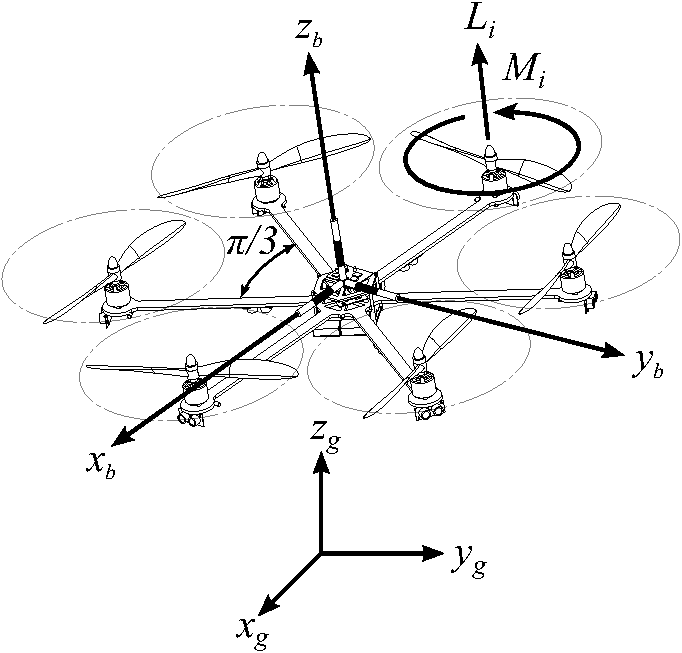
\includegraphics[scale=0.55]{ch3/img/hexacopter_kine.pdf}
	\caption{Hexa--copter kinematics}
\end{figure}
\myparagraph{External force and torque analysis}
There are several force that act on the body of the drone:
\begin{equation}
\totforcehexa_b = \sum\limits_{\mathrm{external}} F_b
\end{equation}

\textbf{Weight}:
\begin{equation}
\mathbf{P}_g = \vettore{0 \\ 0 \\ - m g}
\end{equation}

\textbf{Motor thrust}:
\begin{equation}
\mathbf{L}_b = \sum\limits_{i=1}^6 \vettore{0 \\ 0 \\ -L_{b,i}}
\end{equation}

\textbf{Total force}:
\begin{equation}
\totforcehexa_b = \vettore{\sin(\theta) \\ -\sin(\phi)\cos(\theta) \\ - \cos(\phi)\cos(\theta)} m g + \vettore{ 0 \\ 0 \\ - \sum\limits_{i=1}^6 L_{b,i}}
\end{equation}

For what concerns total external torque applied to the system:
\begin{equation}
\tottorquehexa_{b,\mathbf{0}} = \sum\limits_{\mathrm{external}} M_b + \sum\limits_{\mathrm{external}} (\mathbf{p}_b - \mathbf{0}) \times \totforcehexa_b
\end{equation}

\textbf{Thrust torque}, with $l$ distance between center of propeller and CoM
\begin{equation}
\mathbf{M}_b = \sum\limits_{i=0}^5 \vettore{ l \cos(i \pi/3) \\ l \sin(i \pi /3) \\ 0 } \times \mathbf{L}_{b,i}
\end{equation}

\textbf{Drag torque}, with $\beta$ the proportional factor between thrust and drag torque
\begin{equation}
\mathbf{D}_b = \sum\limits_{i=1}^6 \vettore{ 0 \\ 0 \\ \beta L_{b,i}}
\end{equation}

In general, the total torque is:
\begin{equation}
\tottorquehexa_{b,0} = \left[ \begin{array}{c}
-\dfrac{\sqrt{3}}{2} l \left( L_2 +L_3 - L_5 - L_6 \right) \\
\dfrac{1}{2} l \left( 2 L_1 + L_2 -L_3 - 2 L_4 - L_5 + L_6 \right) \\ 
\beta \left( L_1 - L_2 + L_3 - L_4 + L_5 - L_6 \right)
\end{array}
\right]
\end{equation}

\myparagraph{Inertial analysis}
We could define speed vector in body system of coordinates:
\begin{equation}
\vettore{\dot{x} \\ \dot{y} \\ \dot{z}} = \rotmat \vettore{u\\v\\w}
\end{equation}
\marginnote{The rotational matrix form body to ground is obtained through a sequence of elementary rotations:
${\mathcal{R} = \mathcal{R}_z(\psi)\;\mathcal{R}_y(\theta)\;\mathcal{R}_x(\phi)}$}.  that allows us to define the accelerations vector in the form:
\begin{equation}
\mathbf{a}_b = \dot{\mathbf{v}}_b + \boldsymbol{\omega}_b \times \mathbf{v}_b
\end{equation}
The relation that connects angular ratios in body coordinates and ground coordinates are derived from the so called \emph{Gimball's relations}\sidenote{Just a clarification on the notation used. Square parentheses $[\cdot]$ identifies vector element that belongs to the same basis, while vectorial elements in curly brackets $\{\cdot\}$ do not share the same basis}:
\begin{equation}
\boldsymbol{\omega}_b = \mathcal{R}_x (\phi) \dot{\phi} \vers{e}''_x + \mathcal{R}_x(\phi) \mathcal{R}_y(\theta) \dot{\theta} \vers{e}'_y + \mathcal{R}_x(\phi) \mathcal{R}_y(\theta) \mathcal{R}_z(\psi) \dot{\psi} \vers{e}_z
\end{equation}
that is simplified in the matrix form:
\begin{equation*}
\left[ \begin{array}{c} p \\ q \\ r \end{array} \right] = \left[ \begin{array}{ccc}
 1 & 0 & -\sin(\theta) \\
 0 & \cos(\phi) & \sin(\phi)\cos(\theta) \\
 0 & -\sin(\phi) & \cos(\phi)\cos(\theta)
 \end{array} \right] \left\{ \begin{array}{c} \dot{\phi} \\ \dot{\theta} \\ \dot{\psi} \end{array} \right\}
\end{equation*}
that through inversion gives:
\begin{equation}
\left\{ \begin{array}{c} \dot{\phi} \\ \dot{\theta} \\ \dot{\psi} \end{array} \right\} = 
\left[ \begin{array}{ccc}
 1 & \dfrac{\sin(\phi) \sin(\theta)}{\cos(\theta)} &  \dfrac{\cos(\phi) \sin(\theta)}{\cos(\theta)}\\
 0 & \cos(\phi) & -\sin(\phi) \\
 0 & \dfrac{\sin(\phi)}{\cos(\theta)} & \dfrac{\cos(\phi)}{\cos(\theta)} 
 \end{array} \right]
\left[ \begin{array}{c} p \\ q \\ r \end{array} \right]
\end{equation}
For what concerns angular inertia in body reference frame:
\begin{equation}
\begin{array}{rcl}
\dot{\mathbf{K}}_b &=& \matriceinerzia \dot{\boldsymbol{\omega}}_b + \boldsymbol{\omega}_b \times \matriceinerzia \boldsymbol{\omega}_b \\
&=& \left[ \begin{array}{c} I_x \dot{p} \\ I_y \dot{q} \\ I_z \dot{r} \end{array} \right] + \left[ \begin{array}{c} (I_z-I_y) q r \\ (I_x-I_z) p r \\ (I_y-I_x) p q \end{array} \right]
\end{array}
\end{equation}

\myparagraph{Newton--Euler equations}
Defined state vectors and control vectors:
\arraymath{%
\hexastate & = & \left[ x,y,z,u,v,w,\phi,\theta,\psi,p,q,r \right]^T \\
\hexacontrol & = & \left[ L_1, L_2, L_3, L_4, L_5, L_6 \right]^T%
}
we get the following Newton--Euler equations that describes dynamical behavior of the drone:
\begin{equation}
\left\{\begin{array}{rcl}
\dot{x} &=&\cos ( \psi) \cos ( \theta) u +\sin ( \psi) \cos ( \theta) v -\sin ( \theta) w \\
\dot{y} &=& \cos ( \psi ) u \sin ( \theta ) \sin ( \phi) +\sin( \psi) v \sin ( \theta) \sin ( \phi ) + \\ & &  +\cos ( \psi) v  \cos ( \phi) +\cos ( \theta) \sin ( \phi ) w -u \sin ( \psi) \cos ( \phi) \\
\dot{z} & = &\cos ( \psi) u \sin ( \theta ) \cos ( \phi) +\sin( \psi) v \sin ( \theta) \cos ( \phi ) + \\ & & -\cos ( \psi) v  \sin ( \phi) +\cos (\theta) \cos ( \phi ) w +u \sin ( \psi) \sin ( \phi) \\
\dot{u} & = & - q\;w + r\;v + g \sin(\theta) \\
\dot{v} & = & - r\;u + p\;w - g \sin(\phi) \cos(\theta) \\
\dot{w} & = & - p\;v + q\;u - g \cos(\theta) \cos(\phi) + \\ & &-\dfrac{1}{m} \left(L_1 + L_2 + L_3 + L_4 + L_5 + L_6 \right) \\

\dot{\phi} & = & p + \dfrac{\sin(\phi) \sin(\theta)}{\cos(\theta)}\;q + \dfrac{\cos(\phi) \sin(\theta)}{\cos(\theta)}\;r \\
\dot{\theta} & = & \cos(\phi)\;q - \sin(\phi)\;r \\
\dot{\psi} & = & \dfrac{\sin(\phi)}{\cos(\theta)}\;q + \dfrac{\cos(\phi)}{\cos(\theta)}\;r \\
\dot{p} & = & -\dfrac{I_z-I_y}{I_x} q\;r -\dfrac{\sqrt{3}}{2}\;\dfrac{l}{I_x}\;\left( L_2 +L_3 - L_5 - L_6 \right) \\
\dot{q} & = & -\dfrac{I_x-I_z}{I_y} p\;r + \dfrac{1}{2}\;\dfrac{l}{I_y}\;\left( 2 L_1 + L_2 -L_3 - 2 L_4 - L_5 + L_6 \right) \\
\dot{r} & = & -\dfrac{I_y-I_x}{I_z} p\;q + \dfrac{\beta}{I_z}\;\left( L_1 - L_2 + L_3 - L_4 + L_5 - L_6 \right)
\end{array}\right.
\end{equation}
\begin{margintable}
	\renewcommand{\arraystretch}{1.2}
	\begin{center}
	\begin{tabular}{p{0.5cm} p{2cm} p{1.5cm}}
	\hline \textbf{Sym.} & \textbf{Description} & \textbf{Value} \\ \hline
	$g$     & Gravity        & $9.81 $ \si{\kilo\gram\per\square\second} \\
	$m$     & Mass           & $2$     \si{\kilo\gram}\\
	$I_x$   & $x$ Inertia    & $0.008$ \si{\kilo\gram\square\meter}\\
	$I_y$   & $y$ Inertia    & $0.01$  \si{\kilo\gram\square\meter}\\
	$I_z$   & $z$ Inertia    & $0.05$  \si{\kilo\gram\square\meter}\\
	$\beta$ & Drag parameter & $0.2$   \si{\kilo\gram\square\meter}\\
	$l$     & Frame arm      & $0.3$   \si{\meter} \\ \hline
	\renewcommand{\arraystretch}{1.75}
	\end{tabular}
	\end{center}
	\caption{Mechanicals parameters of the simulated model}
\end{margintable}

\subsection{Linearization and LQR control}
\myparagraph{Linearization}
We now linearize the system feedback to get a control that stabilizes our drone:
\begin{equation}
\hexacontrol_0 \; : \; \mathbf{0}=f(\hexastate_0, \hexacontrol_0)
\end{equation}
that will be solved for hovering state, that is one of the most important flight routine. In a drone, hovering is not dependent with respect to vertical orientation along $\vers{z}$ axis:
\[
\hexastate = \left[ x_0, y_0, z_0,0,0,0,0,0,\psi_0,0,0,0 \right]^T
\]
One solution for this state is the control vector composed by thrust forces:
\[
L_1 = L_2 = L_3 = L_4 = L_5 = L_6 = \dfrac{mg}{6}
\]
and the linearized system is in the form:
\begin{equation}
\dot{\hexastate} = \underset{A}{\underbrace{\dfrac{\partial f(\hexastate,\hexacontrol)}{\partial \hexastate} \Big\rfloor_{\hexastate_0,\hexacontrol_0}}} \hexastate + \underset{B}{\underbrace{\dfrac{\partial f(\hexastate,\hexacontrol)}{\partial \hexacontrol} \Big\rfloor_{\hexastate_0,\hexacontrol_0}}} \hexacontrol
\end{equation}
and it is possible to obtain a representation of a linear model using a computer algebra system:
\renewcommand{\arraystretch}{1}
\begin{equation}
A = \left[ \begin{array}{cccccccccccc} 0&0&0&\cos \left( \psi_{{0}}
 \right) &\sin \left( \psi_{{0}} \right) &0&0&0&0&0&0&0
\\  0&0&0&-\sin \left( \psi_{{0}} \right) &\cos
 \left( \psi_{{0}} \right) &0&0&0&0&0&0&0\\  0&0&0&0&0
&1&0&0&0&0&0&0\\  0&0&0&0&0&0&0&g&0&0&0&0
\\  0&0&0&0&0&0&-g&0&0&0&0&0\\  0&0&0
&0&0&0&0&0&0&0&0&0\\  0&0&0&0&0&0&0&0&0&1&0&0
\\  0&0&0&0&0&0&0&0&0&0&1&0\\  0&0&0
&0&0&0&0&0&0&0&0&1\\  0&0&0&0&0&0&0&0&0&0&0&0
\\  0&0&0&0&0&0&0&0&0&0&0&0\\  0&0&0
&0&0&0&0&0&0&0&0&0\end{array} \right]
\end{equation}
\begin{equation}
B = \left[ \begin {array}{cccccc} 0&0&0&0&0&0\\  0&0&0&0
&0&0\\  0&0&0&0&0&0\\  0&0&0&0&0&0
\\  0&0&0&0&0&0\\   -\dfrac{1}{m}& -\dfrac{1}{m}& -\dfrac{1}{m}& -\dfrac{1}{m}& -\dfrac{1}{m}& -\dfrac{1}{m}\\  0&0&0&0
&0&0\\  0&0&0&0&0&0\\  0&0&0&0&0&0
\\  0&-\dfrac{\sqrt{3}}{2}\dfrac{l}{I_x}&-\dfrac{\sqrt{3}}{2}\dfrac{l}{I_x}&0&
\dfrac{\sqrt{3}}{2}\dfrac{l}{I_x}&\dfrac{\sqrt{3}}{2}\dfrac{l}{I_x}\\  \dfrac{l}{I_y}&\dfrac{1}{2}\dfrac{l}{I_y}&-\dfrac{1}{2}\dfrac{l}{I_y}&-\dfrac{l}{I_y}&-\dfrac{1}{2}\dfrac{l}{I_y}&\dfrac{1}{2}\dfrac{l}{I_y}
\\  \dfrac{\beta}{I_z}&-\dfrac{\beta}{I_z}&\dfrac{\beta}{I_z}&-\dfrac{\beta}{I_z}&\dfrac{\beta}{I_z}&-\dfrac{\beta}{I_z} \end {array} \right]
\end{equation}
\renewcommand{\arraystretch}{1.75}

\myparagraph{LQR on complete state}
From our linear system:
\begin{equation}
\dot{\hexastate} = A \hexastate + B \hexacontrol
\end{equation}
given the quadratic control cost function, with infinite horizon:
\[
J = \int\limits_{0}^{\infty} \hexastate^T Q \hexastate + \hexacontrol^T R \hexacontrol\, dt
\]
with $Q$ and $R$ positive defined.The optimum control that minimize this functional is: 
\begin{equation}
\hexacontrol^* = - R^{-1} B^T P \hexastate
\end{equation}
where $P$ is the solution of \emph{Riccati's equation}:
\[
A^T P + PA - P B R^{-1} B^T P + Q = 0
\]
\begin{margintable}
\renewcommand{\arraystretch}{1}
	\begin{centering}
	\begin{tabular}{p{1.5cm} p{1.5cm}}
		\hline
		\textbf{Parameter} & \textbf{Value} \\
		\hline
		$q_1$    & $10$ \\
		$q_2$    & $10$ \\
		$q_3$    & $2.5$ \\
		$q_4$    & $0.01$ \\
		$q_5$    & $0.01$ \\
		$q_6$    & $0.01$ \\
		$q_7$    & $20$ \\
		$q_8$    & $20$ \\
		$q_9$    & $10$ \\
		$q_{10}$ & $15$ \\
		$q_{11}$ & $15$ \\
		$q_{12}$ & $5$ \\
		$\rho$   & $1$ \\ \hline
	\end{tabular}
	\end{centering}
	\caption{Functional weights}
\renewcommand{\arraystretch}{1.75}	
\end{margintable}
the solution of this equation is obtain through numerical tools such as Matlab's \texttt{lqr} algorithm. Unfortunately it is impossible to derive analytical solution, given a wise chose of $Q$ and $R$ matrix. Usually, and also in this case, it is a good idea to follow the Bryson estimation (diagonal matrix, with higher weight to $Q$ matrix, or \emph{cheap control}):
\[
\begin{array}{rcl}
Q & = & \mathrm{eye}\left( q_i \; : \; i = 1..12 \right) \\
R & = & \rho \mathbb{I}_{6\times 6}
\end{array}
\]
whit the additional constraint to keep observability and controllability on couples:
\[
\begin{array}{rcl}
\mathcal{O}\braces{A,\sqrt{Q}} & = & \mathrm{rank}\braces{ \sqrt{Q}^T\;A^T\sqrt{Q}^T\;\dots\;\braces{A^T}^{\dim(\hexastate)-1}\sqrt{Q}^T} = 12 \\
\mathcal{C}\braces{A,B} & = & \mathrm{rank}\braces{ B\;A B\;\dots\;\braces{A}^{\dim(\hexastate)-1}B} = 6
\end{array}
\]

\myparagraph{Solving tracking problem}
\begin{marginfigure}
	\centering
	%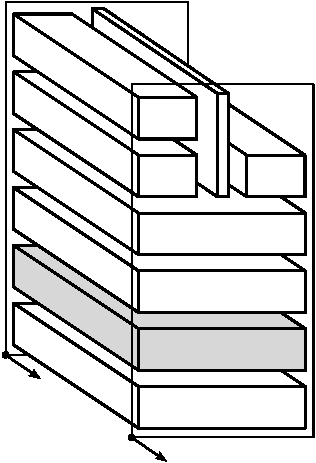
\includegraphics[scale=0.5]{ch3/img/PA_map_tracking.pdf}
	\begin{tikzpicture}[>=latex',scale=0.4]
	\drawplanexy{-0.3}{-0.3}{-0.3}{6.7}{10}{dashed}{perception}
	
	\drawcube{0}{0}{5}{6.4}{1}{white}{dinamica}{}{};
	\drawcube{0}{1.2}{5}{6.4}{1}{gray!40}{tracking}{}{};
	
	\drawcube{0}{2.4}{5}{6.4}{1}{white}{ostacoli}{}{};
	\drawcube{0}{3.6}{5}{6.4}{1}{white}{altitude}{}{};
	
	\drawcube{0}{4.8}{5}{3}{1.5}{white}{source}{}{};
	\drawcube{0}{6.5}{5}{3}{1.5}{white}{emulatore}{}{};

	\drawplanezy{3.2}{4.8}{5}{4.5}{radar_det}{fill=white,opacity=0.90}{}{};

	\drawcube{3.4}{4.8}{5}{3}{3.2}{white}{alpha}{}{};
	\drawplanexy{-0.3}{-0.3}{5.3}{6.7}{10}{dashed}{action}
	

	\draw [->,line width=1.5] (action_D) -- ++(0,0,2);
	\draw [->,line width=1.5] (perception_D) -- ++(0,0,2);

	\coordinate [at=(radar_det_D), yshift=-5] (arrows_point);
	\draw [->,dashed]  (arrows_point) -- ++(1.5,0,0); 
	\draw [->,dashed]  (arrows_point) -- ++(-1.5,0,0); 
\end{tikzpicture}
\end{marginfigure}
It is really simple to solve a tracking problem starting from an LQR, that tries always to reach a zero. Simply insert an offset in position, and the system will try to reduce the error until it reach zero. Here we have a figure that explains the complete control, and some simulation test for random initial conditions that tries to reach a specific position in space.
\begin{figure}
\centering
\begin{tikzpicture}[auto, node distance=2cm,>=latex']
    % Placing blocks
    \node [block] (force) {$L_i = \dfrac{mg}{6}$};
    \node [sum, right of=force] (sumforce) {};
    \node [block, right of=sumforce] (hexacopter) {$\dot{\hexastate}=f(\hexastate,\hexacontrol)$};
    \node [block, right of=hexacopter] (integrator) {$\dfrac{1}{s}$};

    \node [output, right of=integrator] (output) {};

    % draw the lines
    \draw [->] (force) -- node[pos=0.99] {} (sumforce);
    \draw [->] (sumforce) -- node {$\hexacontrol$} (hexacopter);
    \draw [->] (hexacopter) -- node {} (integrator);
    \draw [->] (integrator) -- node [name=x] {$\hexastate$} (output);
    
    \node [sum, below of=x] (sumpos) {};
    \node [block, right of=sumpos] (reachpoint) {$\hexastate_f$};
    \node [gain, left of=sumpos] (gain) {$K$};

    \draw [->] (x) -- (sumpos);
    \draw [->] (reachpoint) -- node[pos=0.99] {$-$} (sumpos);
    \draw [->] (gain) -| node [pos=0.99] {$-$} node [pos=0.2] {$\hexacontrol*$} (sumforce);
    \draw [->] (sumpos) -- node {$\mathbf{e}$} (gain);
\end{tikzpicture}
\caption{Control block scheme}
\end{figure}
\FloatBarrier